\documentclass[11pt]{article}

\usepackage[margin=1in]{geometry}
\usepackage{amsmath,amssymb,mathtools}
\usepackage{graphicx}
\usepackage{xcolor}
\usepackage{booktabs}
\usepackage{microtype}
\usepackage{hyperref}
\usepackage{fancyhdr}
\usepackage{enumitem}

\definecolor{primary}{HTML}{168AAD}
\definecolor{secondary}{HTML}{3F7F2F}
\definecolor{accent}{HTML}{A67C00}
\definecolor{verify}{HTML}{B63E42}

\hypersetup{
  colorlinks=true,
  linkcolor=primary,
  urlcolor=primary,
  pdftitle={Understanding the Integral of x Squared},
  pdfsubject={A companion paper to the Manim explainer video}
}

\pagestyle{fancy}
\fancyhf{}
\lhead{Understanding $\int x^2\,dx$}
\rhead{Video Companion Paper}
\cfoot{\thepage}
\setlength{\headheight}{14pt}

\title{\textbf{Understanding the Integral of $x^2$}\\
\large Geometry, the Power Rule, and Verification}
\author{Companion paper for the Manim explainer video}
\date{}

\begin{document}
\maketitle

\begin{abstract}
This paper explains in detail why
\[
\boxed{\displaystyle \int x^2\,dx=\frac{x^3}{3}+C.}
\]
The explanation follows the visual story in the accompanying animation. We first interpret integration as accumulated area under the parabola $y=x^2$. We then calculate that area using a Riemann sum, connect it to the Fundamental Theorem of Calculus, apply the power rule for antiderivatives, explain the constant of integration, and verify the result by differentiation. Common mistakes and useful generalizations are included at the end.
\end{abstract}

\tableofcontents

\section{The problem and what an indefinite integral means}

We want to evaluate
\[
\int x^2\,dx.
\]
An \emph{indefinite integral} asks for every function whose derivative equals the integrand. In other words, we seek a function $F$ such that
\[
F'(x)=x^2.
\]
Such a function is called an \emph{antiderivative} of $x^2$. This reverses differentiation: differentiation starts with a function and computes its rate of change, while antidifferentiation starts with a rate of change and reconstructs a possible original function.

The answer is not a single function. If $F'(x)=x^2$, then for every real constant $C$,
\[
\frac{d}{dx}\bigl(F(x)+C\bigr)=F'(x)+0=x^2.
\]
Therefore, an indefinite integral must describe a whole family of functions. That is why its final form includes $+C$.

\section{The geometric meaning: accumulated area}

For nonnegative $x$, the graph $y=x^2$ lies on or above the horizontal axis. The definite integral
\[
A(a)=\int_0^a x^2\,dx, \qquad a\ge 0,
\]
measures the area between the parabola, the $x$-axis, and the vertical lines $x=0$ and $x=a$.

\begin{figure}[ht]
  \centering
  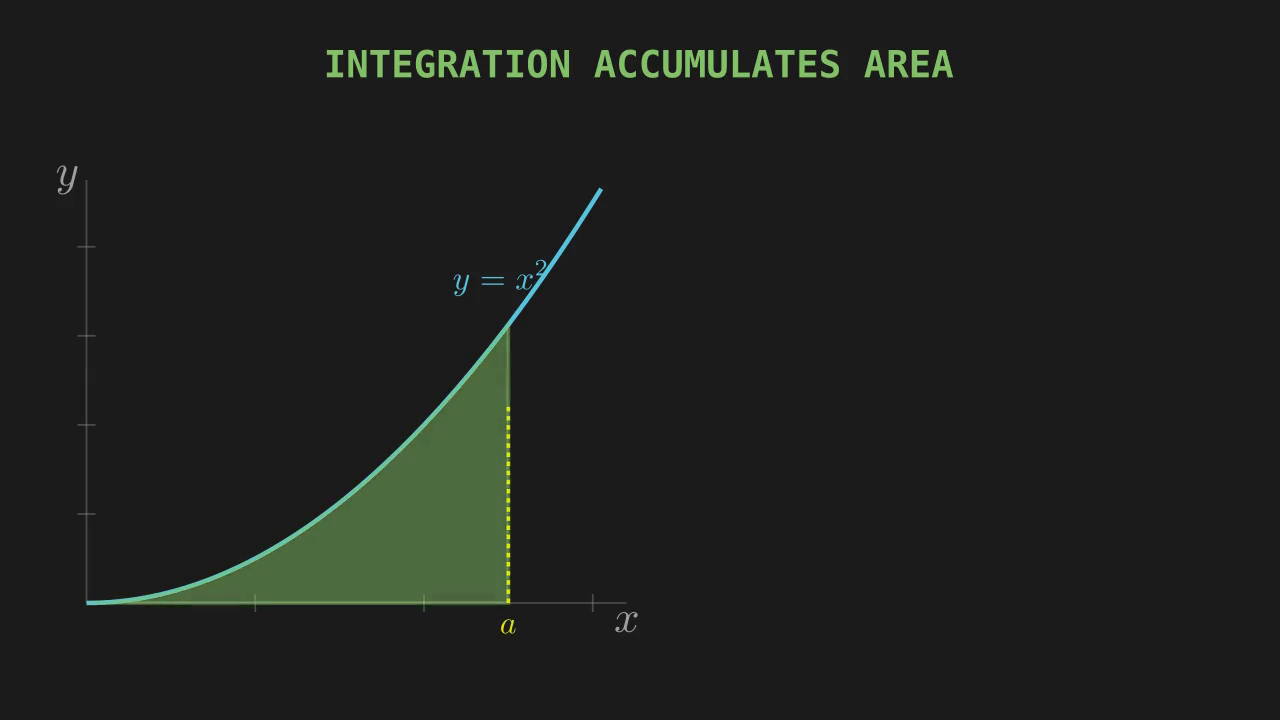
\includegraphics[width=0.83\textwidth]{assets/geometry.png}
  \caption{A frame from the video: the green region represents the accumulated area under $y=x^2$ from $0$ to $a$.}
  \label{fig:area}
\end{figure}

As $a$ increases, two quantities change:
\begin{itemize}[leftmargin=2em]
  \item the width of the interval $[0,a]$ increases;
  \item the height of the parabola at the moving endpoint is $a^2$.
\end{itemize}
The area therefore grows faster and faster. The resulting area function is cubic:
\[
A(a)=\frac{a^3}{3}.
\]
The next section proves this statement directly from rectangular approximations.

\section{Computing the area with a Riemann sum}

Divide $[0,a]$ into $N$ subintervals of equal width
\[
\Delta x=\frac{a}{N}.
\]
Using right endpoints, the $k$th sample point is
\[
x_k=\frac{ka}{N}, \qquad k=1,2,\ldots,N.
\]
The corresponding rectangle has height
\[
f(x_k)=x_k^2=\left(\frac{ka}{N}\right)^2.
\]
Its area is height times width:
\[
f(x_k)\Delta x
=\left(\frac{ka}{N}\right)^2\frac{a}{N}
=\frac{k^2a^3}{N^3}.
\]
Summing all rectangles gives
\begin{align*}
S_N
&=\sum_{k=1}^{N}\frac{k^2a^3}{N^3}\\
&=\frac{a^3}{N^3}\sum_{k=1}^{N}k^2.
\end{align*}
Using
\[
\sum_{k=1}^{N}k^2=\frac{N(N+1)(2N+1)}{6},
\]
we obtain
\begin{align*}
S_N
&=\frac{a^3}{N^3}\cdot\frac{N(N+1)(2N+1)}{6}\\
&=\frac{a^3}{6}\left(1+\frac{1}{N}\right)
  \left(2+\frac{1}{N}\right).
\end{align*}
Taking the limit as the rectangles become infinitely thin,
\begin{align*}
\int_0^a x^2\,dx
&=\lim_{N\to\infty}S_N\\
&=\frac{a^3}{6}(1)(2)\\
&=\boxed{\frac{a^3}{3}}.
\end{align*}
Thus the geometric area calculation already suggests that an antiderivative of $x^2$ is $x^3/3$.

\section{The power rule for antiderivatives}

The same result can be obtained more efficiently using the power rule. For any real exponent $n\ne -1$,
\[
\boxed{\displaystyle \int x^n\,dx=\frac{x^{n+1}}{n+1}+C.}
\]
This rule has two operational steps:
\begin{enumerate}[leftmargin=2em]
  \item increase the exponent by one;
  \item divide by the new exponent.
\end{enumerate}

For $x^2$, the old exponent is $2$. Increasing it by one gives $3$, and dividing by the new exponent gives
\begin{align*}
\int x^2\,dx
&=\frac{x^{2+1}}{2+1}+C\\
&=\boxed{\frac{x^3}{3}+C}.
\end{align*}

\subsection{Why the power rule works}

The formula is not arbitrary. It is designed to reverse the derivative power rule. Differentiate the proposed antiderivative:
\begin{align*}
\frac{d}{dx}\left(\frac{x^{n+1}}{n+1}\right)
&=\frac{1}{n+1}\frac{d}{dx}\left(x^{n+1}\right)\\
&=\frac{1}{n+1}(n+1)x^n\\
&=x^n.
\end{align*}
The factor $n+1$ created by differentiation cancels the denominator $n+1$. This cancellation explains both parts of the integration rule.

The restriction $n\ne -1$ is essential because division by $n+1$ would otherwise mean division by zero. The exceptional case is
\[
\int \frac{1}{x}\,dx=\ln|x|+C,
\]
not a power of $x$.

\section{The constant of integration}

The expression
\[
\frac{x^3}{3}+C
\]
represents infinitely many vertically shifted cubic curves. For example,
\[
\frac{x^3}{3},\qquad \frac{x^3}{3}+5,
\qquad \frac{x^3}{3}-12
\]
all have derivative $x^2$. Differentiation removes every constant, so the integrand alone cannot tell us which vertical shift was the original function.

A definite integral does not need an arbitrary $C$ in its final numerical value because the constants cancel at the endpoints:
\begin{align*}
\int_0^a x^2\,dx
&=\left[\frac{x^3}{3}+C\right]_0^a\\
&=\left(\frac{a^3}{3}+C\right)-\left(0+C\right)\\
&=\frac{a^3}{3}.
\end{align*}
This agrees exactly with the Riemann-sum area calculation.

\section{Verification by differentiation}

The safest way to check an indefinite integral is to differentiate the answer. Starting from
\[
F(x)=\frac{x^3}{3}+C,
\]
we calculate
\begin{align*}
F'(x)
&=\frac{d}{dx}\left(\frac{x^3}{3}+C\right)\\
&=\frac{1}{3}\cdot 3x^2+0\\
&=x^2.
\end{align*}
The derivative reproduces the original integrand, so the antiderivative is correct.

\begin{figure}[ht]
  \centering
  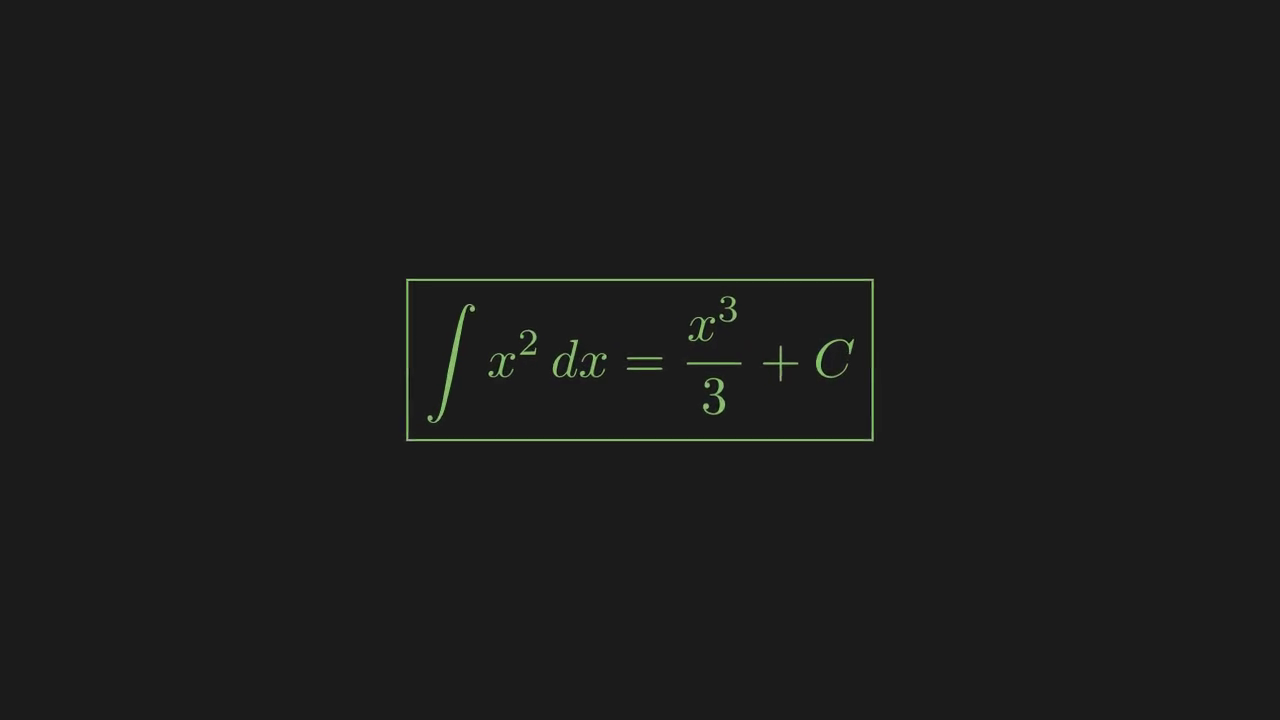
\includegraphics[width=0.72\textwidth]{assets/final-answer.png}
  \caption{The final result displayed at the end of the animation.}
  \label{fig:answer}
\end{figure}

\section{Connection to the Fundamental Theorem of Calculus}

Define the accumulated-area function
\[
A(a)=\int_0^a x^2\,dx.
\]
The Fundamental Theorem of Calculus states that
\[
A'(a)=a^2.
\]
Geometrically, a small increase $\Delta a$ adds a thin strip whose approximate area is
\[
a^2\Delta a.
\]
Therefore, area changes at a rate approximately equal to the current height of the graph. In the limit, this becomes $A'(a)=a^2$.

Since the Riemann-sum calculation gave $A(a)=a^3/3$, differentiation confirms
\[
A'(a)=\frac{d}{da}\left(\frac{a^3}{3}\right)=a^2.
\]
This is the central link between the geometric and algebraic views: integration accumulates area, while differentiation measures how rapidly that accumulated area changes.

\section{Common mistakes}

\begin{center}
\begin{tabular}{p{0.39\textwidth} p{0.49\textwidth}}
\toprule
\textbf{Mistake} & \textbf{Correction}\\
\midrule
Writing $\int x^2\,dx=x^3+C$ & After raising the exponent, divide by the new exponent: $x^3/3+C$.\\[4pt]
Dividing by the old exponent $2$ & Divide by $2+1=3$, not by $2$.\\[4pt]
Forgetting $+C$ & Every indefinite integral includes an arbitrary constant.\\[4pt]
Treating $dx$ as an exponent & $dx$ identifies the integration variable; it is not part of $x^2$.\\[4pt]
Using the power rule for $x^{-1}$ & The case $n=-1$ is exceptional: $\int x^{-1}dx=\ln|x|+C$.\\[4pt]
Not checking the answer & Differentiate the proposed antiderivative and confirm that the original integrand returns.\\
\bottomrule
\end{tabular}
\end{center}

\section{Generalizations and examples}

The same method applies to any polynomial, term by term. For example,
\begin{align*}
\int \left(4x^3-6x^2+5\right)\,dx
&=4\frac{x^4}{4}-6\frac{x^3}{3}+5x+C\\
&=x^4-2x^3+5x+C.
\end{align*}
Differentiating gives
\[
4x^3-6x^2+5,
\]
which verifies the result.

For a definite example,
\begin{align*}
\int_0^2 x^2\,dx
&=\left[\frac{x^3}{3}\right]_0^2\\
&=\frac{2^3}{3}-\frac{0^3}{3}\\
&=\frac{8}{3}.
\end{align*}
This is the exact area under $y=x^2$ from $x=0$ to $x=2$.

\section{Summary}

The integral of $x^2$ can be understood from several mutually reinforcing viewpoints:
\begin{enumerate}[leftmargin=2em]
  \item \textbf{Antiderivative viewpoint:} find a function whose derivative is $x^2$.
  \item \textbf{Geometric viewpoint:} accumulate area under the parabola $y=x^2$.
  \item \textbf{Riemann-sum viewpoint:} the limit of rectangular approximations from $0$ to $a$ is $a^3/3$.
  \item \textbf{Power-rule viewpoint:} raise the exponent from $2$ to $3$ and divide by $3$.
  \item \textbf{Verification viewpoint:} differentiating $x^3/3+C$ returns $x^2$.
\end{enumerate}
All of these lead to the same conclusion:
\[
\boxed{\displaystyle \int x^2\,dx=\frac{x^3}{3}+C.}
\]

\end{document}
